% !TEX root = chapter-standalone.tex

\section{Monotone functions}
\label{sec:monotonicity-monotone-maps}

%\linkvideo{spring2021-functors:semi-and-fun:mon-functions} % Monotone functions
% \linkvideo{spring2021-functors:semi-and-fun:mon-functions:fun-req-mon} % Functionalities and requirements
\linkvideo{spring2021-functors:semi-and-fun:mon-functions:mon-on-pos} % Monotone functions on posets

A \SY{monotone function} is the generalization to \SY{preorders} of a ``non-decreasing'' function on real numbers.
The function~$\ela \mapsto \max(0, 42 \ela)$ is non-decreasing on the real numbers because
\begin{equation}\label{eq:monotone-eq-1}
    \prfperiod{
        \ela \leq \elb
    }{
        \max(0, 42 \ela) \leq \max(0, 42 \elb)
    }
\end{equation}
Note that we use ``$\leq$'' and not ``$<$''.
``Non-decreasing'' is a weaker condition than ``increasing''.

The definition of \SY{monotone function} on a \SY{preorder} is the direct generalization of this concept; the only change is that we use the preorders at hand, rather than the total order on the reals.

\begin{definition}[monotone function]
    \label{def:monotone}
    A \maindef{monotone function} between two \SY{preorders}~$\posAdefinition$ and~$\posBdefinition$ is a function~$\mapa \colon \posAset \sto \posBset$ that is compatible with the preorder relations on its source and target in the sense that
    \begin{equation}\label{eq:monotone-map-definition}
        \prfperiod{
            \posela \posAleq \poselb
        }{
            \mapa(\posela) \posBleq \mapa(\poselb)
        }
    \end{equation}
\end{definition}

\begin{example}[The identity is monotone]
    Given a preorder~\posA, the identity function~$\catidat{\posAset}\colon \posAset \mto\linebreak[0] \posAset$ is a monotone function, since if~$\posela\posAleq \poselb$, then~$\mapidat{\posAset}(\posela)=\posela \posAleq \poselb = \mapidat{\posAset}(\poselb )$.
\end{example}

\begin{example}[Constant functions]
    Every constant function is a monotone function.
\end{example}

\begin{figure*}[b]
    \centering
    \includesag{40_dpcatfig_exmonotone}
    \caption{The cardinality function is a \SY{monotone function}.}
    \label{fig:cardinality}
\end{figure*}

\begin{example}[Cardinality function]\label{exa:cardinality}
    Consider the power \SY{poset} (\cref{def:power-poset}) $\powerposet\setA$ of a finite set \setA.
    The cardinality function
    \begin{equation}\label{eq:cardinality-map}
        \cardmap : \powerset\setA \sto \natnumbers
    \end{equation}
    is monotone when considered as a function from the \SY{poset} $\powerposet\setA$ to the \SY{poset} $\natswithleq$.
    % \begin{equation}
    %     \defmap{
    %         \cardmap
    %     }{
    %         \powerposet{\setA}
    %     }{
    %         \sto
    %     }{
    %         \tup{\natnumbers,\leq}
    %     }{
    %         \subA
    %     }{
    %         \vert\subA\vert
    %     }
    % \end{equation}
    % is monotone.
    \Cref{fig:cardinality} shows a visualization of this function for the set~$\setA=\makeset{\posela,\poselb,\poselc}$.
    To prove this, recall that in the power \SY{poset} subsets are ordered by inclusion.
    Therefore, we need to show that
    \begin{equation}\label{eq:cardinality}
        \prfperiod{
            \subA \setsubseteq \subB
        }{
            \cardof \subA \leq \cardof \subB
        }
    \end{equation}

    This is easy to see that, because all elements of $\subA$ are also in $\subB$, the cardinality of~$\subA$ cannot be more than the cardinality of~$\subB$.
    Monotonicity depends on the preorder relations used on the domain and the codomain.
    To indicate that a function is monotone, we write it indicating the two \SY{preorders} as the domain/codomain:
    \begin{equation}\label{eq:cardinality-as-posmap}
        \cardmap \colon \tup{\powerset\setA, \setsubseteq} \mto \tup{\natnumbers, {{\Nleq}}}.
    \end{equation}
\end{example}

\begin{lemma}
    Let~\posA be a \SY{preorder}.
    The \SY{upper closure} operator~$\upit$ is a \SY{monotone function}
    \begin{equation}
\upit \colon \tupp{\posPA, \setsubseteq} \mto \tupp{\setOfUppersets \posA,{{\setsubseteq}}}.
\end{equation}
\end{lemma}
\begin{proof}
    First, by \cref{lem:upper-closure-is-upper-set},~$\upit \setA$ is an \SY{upper set} for every~$\setA \setin \posPA$, so~$\upit$ is indeed a function with codomain~$\setOfUppersets \posA$.

    Now let~$\setA\com \setB \setin \linebreak[1] \posPA$ with~$\setA\setsubseteq \setB$.
    We must show that~$\upit \setA \setsubseteq \upit \setB$.
    Let~$\styleelements{y}\setin \upit \setA$.
    By definition of~$\upit \setA$, there exists an~$\styleelements{x}\setin \setA$ such that~$\styleelements{x}\posAleq \styleelements{y}$.
    Since~$\setA\setsubseteq \setB$, we also have~$\styleelements{x}\setin \setB$.
    So there exists an element of~$\setB$, namely~$\styleelements{x}$, such that~$\styleelements{x}\posAleq \styleelements{y}$; by definition of~$\upit \setB$, this means~$\styleelements{y}\setin \upit \setB$.
    As~$\styleelements{y}$ was an arbitrary element of~$\upit \setA$, this shows~$\upit \setA \setsubseteq \upit \setB$, as was to be shown.
\end{proof}

\begin{lemma}
    \label{lem:lower_closure_monotone}
    Let~\posA be a \SY{preorder}.
    The \SY{lower closure} operator~
    \begin{equation}
    \downit \colon \tupp{\posPA, \setsubseteq}  \to \tupp{\setOfLowersets \posA, \setsubseteq}
\end{equation}
is a \SY{monotone function}.
\end{lemma}


\begin{gradedexercise}[\exname{LowerClosureMonotone}] 
    Prove \cref{lem:lower_closure_monotone}.
\end{gradedexercise}

\solutionof{LowerClosureMonotone}

\begin{gradedexercise}[\exname{WhichMapsMonotone}] [4 points]

    Consider the posets~$\posA = \tup{\posAset, \posleq_\posA}$ and~$\posB = \tup{\posBset, \posleq_\posB}$ described respectively by the following Hasse diagrams.

    \begin{equation}
        %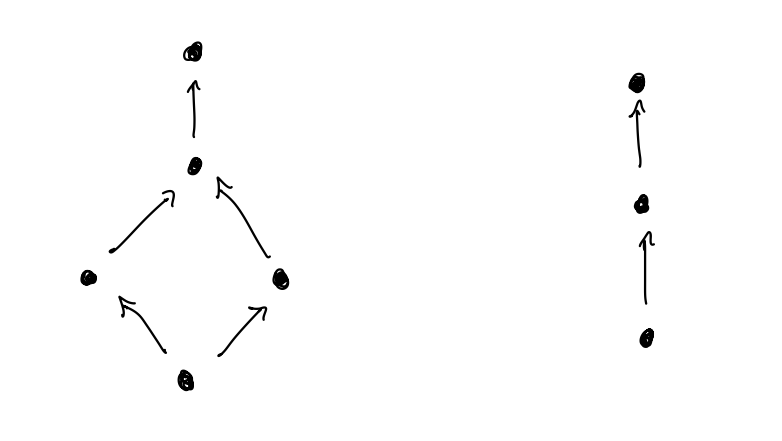
\includegraphics[width=0.5\linewidth]{pics/ExamPosets.png}
        \includesag{exam_posets}
    \end{equation}

    The following diagrams show functions~$\posAset \mto \posBset$.
    We will call them~$\mapaindex{1}$,~$\mapaindex{2}$,~$\mapaindex{3}$ and~$\mapaindex{4}$, respectively.

    \begin{center}
        \setlength{\tabcolsep}{30pt}
        \begin{tabular}{cc}
            $\mapaindex{1}$ &
            %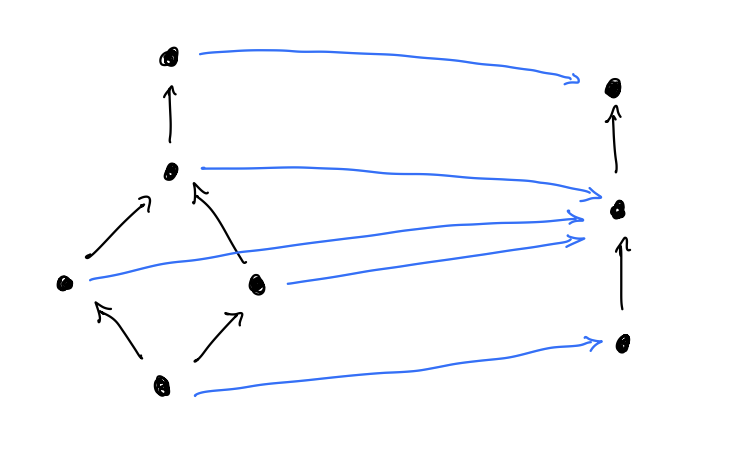
\includegraphics[width=0.5\linewidth]{pics/ExamPosetMap1.png}
            \includesag{exam_f1} \\[+40pt]
            $\mapaindex{2}$ &
            %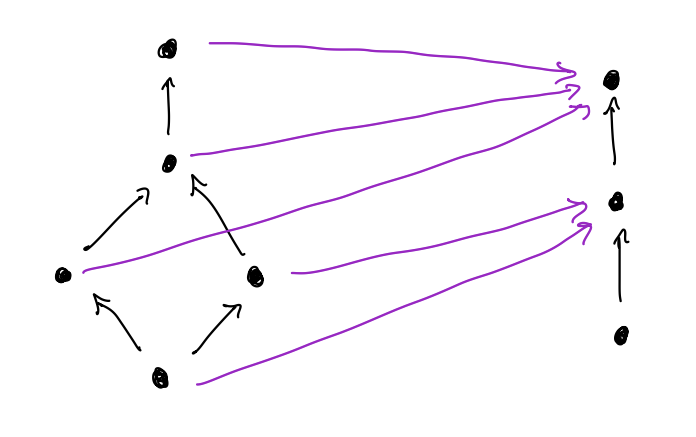
\includegraphics[width=0.5\linewidth]{pics/ExamPosetMap2.png}
            \includesag{exam_f2} \\[+40pt]
            $\mapaindex{3}$ &
            %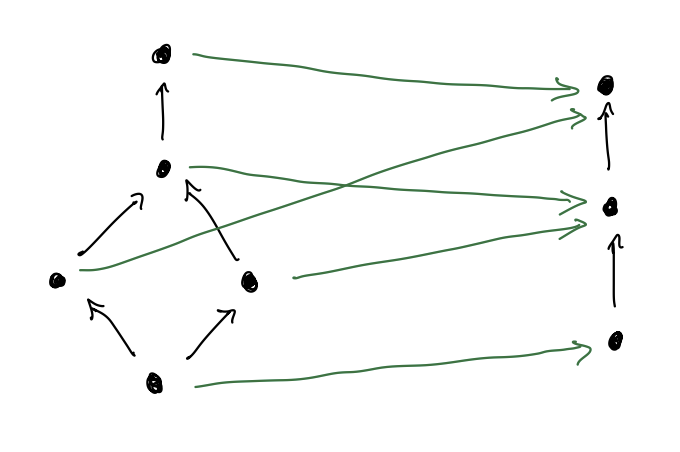
\includegraphics[width=0.5\linewidth]{pics/ExamPosetMap3.png}
            \includesag{exam_f3} \\[+40pt]
            $\mapaindex{4}$ &
            %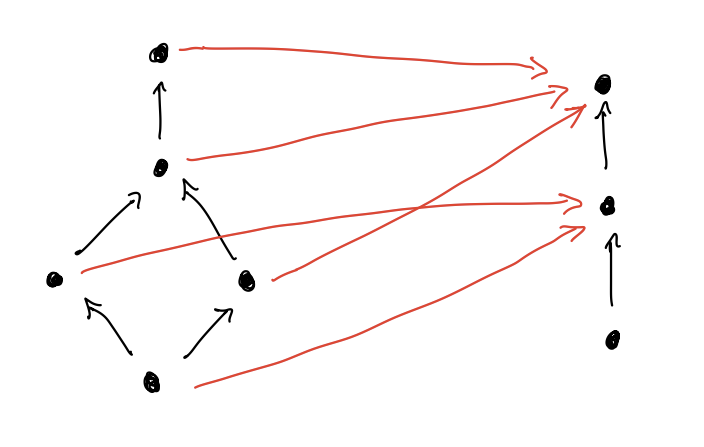
\includegraphics[width=0.5\linewidth]{pics/ExamPosetMap4.png}
            \includesag{exam_f4}
        \end{tabular}
    \end{center}

    Which of the functions~$\mapaindex{1}$,~$\mapaindex{2}$,~$\mapaindex{3}$ and~$\mapaindex{4}$ are monotone functions?
\end{gradedexercise}
\solutionof{WhichMapsMonotone}

\begin{lemma}\label{lem:discrete-is-monotone}
    Consider a discrete poset~\posA and a \SY{preorder}~\posB.
    Any function~$\mapa \colon \posA\to \posB$ is monotone.
\end{lemma}
\newcommand{\samewidth}[1]{\makebox[3cm]{$#1$}}

\begin{gradedexercise}[\exname{FromDiscretePosets}]
    Prove \cref{lem:discrete-is-monotone}
\end{gradedexercise}
\solutionof{FromDiscretePosets}

\clearpage
\vfill
\begin{gradedexercise}[\exname{MonotoneMapCheck}]
    \label{ex:MonotoneMapCheck}

    Prove your answers to the following questions.
    \begin{enumerate}
        \item Is the function
              \begin{equation*}
                  \defmap{\mapa}{\wholewithleq}{\mto}{\wholewithleq}{\ela}{\ela^2}
              \end{equation*}
              monotone?
        \item Let~$\setA = \makeset{\setAel, \setBel, \setCel}$ and consider the posets~$\tup{\powerset{\setA}, \stylemorph{\subseteq}}$ and~$\tup{\natnumbers, \Nleq}$.
              Let
              \begin{equation*}
                  \defmap{\mapa}{\powerset{\setA}}{\to}{\natnumbers}{\subA}{\cardmap(\subA)}
              \end{equation*}
              be the function which calculates the cardinality of any subset of~$\setA$.
              Is~$\mapa$ monotone?
        \item Consider the set of natural numbers which divide the number 36, equipped with the partial order ``$\preccurlyeq$'' such that~$\ela \preccurlyeq \elb$ if and only if~$\ela$ divides~$\elb$.
              Call this poset~$\posA = \tup{\posAset, \preccurlyeq}$, and let~$\mapa \colon \posAset \to \makeset{\false, \true}$ be defined by
              \begin{equation}
                  \mapa(\ela) =
                  \begin{cases}
                      \true  & \text{ if } \ela \text{ is an even number, } \\
                      \false & \text{ if } \ela \text{ is an odd number.
                      }
                  \end{cases}
              \end{equation}
              Is~$\mapa$ monotone if we equip~$\makeset{\false, \true}$ with the usual partial order such that~$\false \preceq \true$?
    \end{enumerate}
\end{gradedexercise}
\solutionof{MonotoneMapCheck}

\begin{ctdefinition}[Order isomorphism]
    \label{def:order-isomorphism}
    A \SY{monotone function}~$\mapa \colon \posA \mto \posB$ between \SY{preorders} is an \maindef{order isomorphism} if~$\mapa$ is \SY{bijective} and, for all~$\posela, \poselb \setin \posAset$,
    \begin{equation}
        \prfdoubleperiod{
            \posela \posleqof\posA \poselb
        }{
            \mapa(\posela) \posleqof\posB \mapa(\poselb)
        }
    \end{equation}
\end{ctdefinition}

\todotext{J: add example of an order isomorphism}

\begin{example}[A bijective monotone function that is not an order isomorphism]
    \label{exa:bijective-monotone-not-iso}
    Let~$\posAset = \makeset{\posela, \poselb}$ be a set with two distinct elements, and consider two different \SY{preorders} with this same underlying set.
    \begin{itemize}
        \item Let~$\posA = \tup{\posAset, {{=}}}$ be the discrete poset on~$\posAset$ (\cref{ex:discreteposet}), in which each element is related only to itself.
        \item Let~$\posB = \tup{\posBset, \posBleq}$, with~$\posBset = \posAset$, be the two-element chain in which~$\posela \posBleq \poselb$ (in addition to~$\posela \posBleq \posela$ and~$\poselb \posBleq \poselb$).
    \end{itemize}
    Consider the identity function~$\mapidat{\posAset}\colon \posAset \sto \posAset$, viewed as a function from~\posA to~\posB.
    \begin{itemize}
        \item It is monotone, by \cref{lem:discrete-is-monotone}, since~\posA is discrete.
        \item It is bijective, since every identity function is.
        \item It is \emph{not} an order isomorphism: we have~$\mapidat{\posAset}(\posela) = \posela \posBleq \poselb = \mapidat{\posAset}(\poselb)$, but~$\posela \posleqof\posA \poselb$ does not hold, because~$\posela \neq \poselb$.
        So the implication from right to left in \cref{def:order-isomorphism} fails.
    \end{itemize}
\end{example}
Therefore, a bijective monotone function need not be an order isomorphism.
Besides being bijective, an order isomorphism must also \emph{reflect} the order: whenever~$\mapa(\posela) \posleqof\posB \mapa(\poselb)$, it must be the case that~$\posela \posleqof\posA \poselb$.

\subsection{Monotonicity is compositional}

\SY{Monotonicity} is a compositional property: the series composition of two \SY{monotone functions} is \SY{monotone}.
\begin{lemma}\label{lem:monotonicity-compositional}
    Given \SY{preorders}~$\posA,\posB,\posC$ and two \SY{monotone functions}
    $\mapa\colon \posA \mto \posB$ and $\mapb\colon \posB \mto \posC$, the composite function~$\mapa\mthen \mapb\colon \posA \mto \posC$ is monotone as well.
\end{lemma}
\begin{proof}
    Let~$\posAnel{1},\posAnel{2} \setin \posAset$ with~$\posAnel{1}\posAleq \posAnel{2}$.
    We must show that~$(\mapa\mthen \mapb)(\posAnel{1}) \posCleq (\mapa\mthen \mapb)(\posAnel{2})$.
    Since~$\mapa$ is \SY{monotone}, we have
    %
    \begin{equation}\label{eq:monotonicity-compositional-1}
        \mapa(\posAnel{1})\posBleq \mapa(\posAnel{2}).
    \end{equation}
    %
    Now~$\mapa(\posAnel{1})$ and~$\mapa(\posAnel{2})$ are two elements of~$\posBset$, and \cref{eq:monotonicity-compositional-1} says that they are related in~\posB.
    Since~$\mapb$ is \SY{monotone}, we can apply its monotonicity condition to these two elements, and obtain
    %
    \begin{equation}\label{eq:monotonicity-compositional-2}
        \mapb(\mapa(\posAnel{1}))\posCleq \mapb(\mapa(\posAnel{2})).
    \end{equation}
    %
    By definition of composition,~$(\mapa\mthen \mapb)(\posela) = \mapb(\mapa(\posela))$ for every~$\posela \setin \posAset$, so \cref{eq:monotonicity-compositional-2} says precisely that
    %
    \begin{equation}\label{eq:monotonicity-compositional-3}
        (\mapa\mthen \mapb)(\posAnel{1}) \posCleq (\mapa\mthen \mapb)(\posAnel{2}).
    \end{equation}
    %
    Since~$\posAnel{1}$ and~$\posAnel{2}$ were arbitrary elements of~$\posAset$ with~$\posAnel{1}\posAleq \posAnel{2}$, this is the \SY{monotonicity} condition for the composite function~$\mapa\mthen\mapb$.
\end{proof}


\subsection{Antitone functions}

Dually to \SY{monotone functions}, we can define \SY{antitone functions} as order \emph{reversing} functions.

\begin{definition}[Antitone function]
    \label{def:antitone}
    An \maindef{antitone function} between two \SY{preorders}~$\posAdefinition$ and~$\posBdefinition$ is a function~$\mapa$ that reverses the ordering, in the sense that
    \begin{equation}
        \prfperiod{
            \posela \posAleq \poselb
        }{
            \mapa(\posela) \posgeqof\posB \mapa(\poselb)
        }
    \end{equation}
\end{definition}

\begin{example}[Unit cost, total cost]
    Assume that you want to produce some widgets, and that the manufacturing cost depends on the number of widgets.
    The function describing the total cost~$\stylemaps{t}\colon \natnumbers \sto \nonNegReals$ is a function between the ordered sets~\natnumbers and~\nonNegReals, and maps each quantity of widgets to a total manufacturing cost (\cref{fig:total_manufacturing}).
    Clearly,~$\stylemaps{t}$ is a \SY{monotone function}.
    Conversely, the unit cost function~$\stylemaps{u}\colon \natnumbers \sto \nonNegReals$ is antitone (\cref{fig:unit_manufacturing}).
\end{example}

\begin{marginfigure}
    \subfloat[
        Unit cost  \vs  number of widgets.
        \label{fig:unit_manufacturing}
    ]{
        \includesag{unit_manufacturing}
    }

    \subfloat[
        Total cost \vs number of widgets.
        \label{fig:total_manufacturing}
    ]{
        \includesag{total_manufacturing}
    }
    \caption{Unit and total costs vs. number of widgets.}
\end{marginfigure}



It is easy to see that an \SY{antitone function} $\mapa: \posA \mto \posB$ is the same thing as a \SY{monotone function} $\mapa: \posAop \mto \posB$.

\begin{lemma}\label{lem:antitone-is-monotone}
    An \SY{antitone function} $\mapa: \posA \mto \posB$ is a \SY{monotone function} $\mapa: \posAop \mto \posB$
    and a \SY{monotone function} $\mapa: \posA \mto \posB\posop$.
\end{lemma}

